%
% $RCSfile: conceptual_network.tex,v $
%
% Copyright (C) 2002-2008. Christian Heller.
%
% Permission is granted to copy, distribute and/or modify this document
% under the terms of the GNU Free Documentation License, Version 1.1 or
% any later version published by the Free Software Foundation; with no
% Invariant Sections, with no Front-Cover Texts and with no Back-Cover
% Texts. A copy of the license is included in the section entitled
% "GNU Free Documentation License".
%
% http://www.cybop.net
% - Cybernetics Oriented Programming -
%
% http://www.resmedicinae.org
% - Information in Medicine -
%
% Version: $Revision: 1.1 $ $Date: 2008-08-19 20:41:06 $ $Author: christian $
% Authors: Christian Heller <christian.heller@tuxtax.de>
%

\section{Conceptual Network}
\label{conceptual_network_heading}
\index{Conceptual Network}
\index{Ontology}

John F. Sowa \cite{sowa} cites the computer science pioneer Alan Perlis who,
being asked whether a computer could automatically write programs from informal
specifications, replied: \textit{It is not possible to translate informal
specifications to formal specifications by any formal algorithm.} And Sowa
writes on: \textit{English syntax is not what makes the translation difficult.
The difficulty results from the enormous amount of background knowledge that
lies behind every word.}

The structuring of such knowledge is what \emph{Ontologies} shall support. They
are the topic of the following sections and will be of importance for the
knowledge schema introduced in chapter \ref{knowledge_schema_heading}.

%
% $RCSfile: ontos_and_logos.tex,v $
%
% Copyright (C) 2002-2008. Christian Heller.
%
% Permission is granted to copy, distribute and/or modify this document
% under the terms of the GNU Free Documentation License, Version 1.1 or
% any later version published by the Free Software Foundation; with no
% Invariant Sections, with no Front-Cover Texts and with no Back-Cover
% Texts. A copy of the license is included in the section entitled
% "GNU Free Documentation License".
%
% http://www.cybop.net
% - Cybernetics Oriented Programming -
%
% http://www.resmedicinae.org
% - Information in Medicine -
%
% Version: $Revision: 1.1 $ $Date: 2008-08-19 20:41:08 $ $Author: christian $
% Authors: Christian Heller <christian.heller@tuxtax.de>
%

\subsection{Ontos and Logos}
\label{ontos_and_logos_heading}
\index{Ontos and Logos}
\index{Ontology}
\index{Metaphysics}
\index{Agent Communication Language}
\index{ACL}
\index{Semantic Web}
\index{Terminology}

The word \emph{Ontology} stems from ancient Greek language, consisting of the
two subterms \emph{Ontos} and \emph{Logos} which literally mean \emph{Stone} (in
the meaning of \emph{Being}) and \emph{Word} (in the meaning of \emph{Study}).
Thus, ontology designates \emph{the study of the nature of reality}.

Manifold, more detailed definitions are given in literature. They mostly relate
to one of the subjects, \emph{Philosophy} or \emph{Information Technology}
(IT). A philosophical one that can be found in Smith and Welty \cite{smith}
says: Ontology is \emph{the science of what is, of the kinds and structures of
objects, properties, events, processes and relations in every area of reality}.
Since what it means for something \emph{to be} or \emph{to be real} were an
issue beyond what is physically accessible, as Daniel \cite{daniel} writes,
ontological questions were \emph{metaphysical}. \emph{Metaphysics} included not
only the study of being and reality but also \emph{the study of specific kinds
of beings}, such as minds. Metaphysics in general and ontology in particular
were both interested in providing a \emph{Logos}, a rational explanation for
existence. The Dictionary of Philosophy of Mind \cite{pomdictionary}, as
further source, states:

\begin{quote}
    Although the term terms \emph{Ontology} and \emph{Metaphysics} are far from
    being univocal and determinate in philosophical jargon, an important
    distinction seems often enough to be marked by them. What we may call
    ontology is the attempt to say what entities exist. Metaphysics, by
    contrast, is the attempt to say, of those entities, what they are. In
    effect, one's ontology is one's \emph{List} of entities, while one's
    metaphysics is an explanatory theory about the \emph{Nature} of those
    entities.
\end{quote}

Besides rather philosophical descriptions, Eric Little \cite{little} also
quotes a more information science-like definition of Gruber \cite{gruber} for
whom an ontology is an: \textit{explicit specification of a conceptualization}
(of a domain), in other words a \emph{formalisation of domain knowledge}. For
the \emph{Ontology Forum} \cite{ontologyorg}, the key ingredients that made up
an ontology were a \textit{vocabulary of basic terms} and a \textit{precise
specification of what those terms mean}. The \emph{Agent Communication Languages}
(ACL) and \emph{Semantic Web} technologies, introduced in sections
\ref{agent_communication_language_heading} and \ref{semantic_web_heading},
respectively, use ontologies in the same meaning. The borders to
\emph{Terminology} (section \ref{terminology_heading}) are often blurry.

The knowledge schema and new language of chapters \ref{knowledge_schema_heading}
and \ref{cybernetics_oriented_language_heading} may represent entity
information (an ontology) as well as meta information about these (metaphysical
explanations). However, in order to avoid conflicts with philosophy, this work
sticks to Gruber's definition of the term \emph{Ontology}, for the time being,
until it defines it in its own way, in chapter \ref{knowledge_schema_heading}.

%
% $RCSfile: applicability.tex,v $
%
% Copyright (C) 2002-2008. Christian Heller.
%
% Permission is granted to copy, distribute and/or modify this document
% under the terms of the GNU Free Documentation License, Version 1.1 or
% any later version published by the Free Software Foundation; with no
% Invariant Sections, with no Front-Cover Texts and with no Back-Cover
% Texts. A copy of the license is included in the section entitled
% "GNU Free Documentation License".
%
% http://www.cybop.net
% - Cybernetics Oriented Programming -
%
% http://www.resmedicinae.org
% - Information in Medicine -
%
% Version: $Revision: 1.1 $ $Date: 2008-08-19 20:41:05 $ $Author: christian $
% Authors: Christian Heller <christian.heller@tuxtax.de>
%

\subsection{Applicability}
\label{applicability_heading}
\index{Artificial Intelligence}
\index{AI}

The \emph{Ontology Forum} \cite{ontologyorg} writes that ontologies find
applicability in many areas of information systems engineering, for example in
database design, in object systems, in knowledge based systems and within many
application areas such as datawarehousing, knowledge management, computer
supported collaborative working and enterprise integration. Depending on the
nature of the knowledge they were concerned with, communities would differ:

\begin{itemize}
    \item[-] \emph{Artificial Intelligence} (AI): ontologies capture domain
        knowledge, while problem-solving methods capture task knowledge
    \item[-] \emph{Natural Language}: ontologies characterise word meaning and
        sense
    \item[-] \emph{Database}: ontologies, as conceptual schema, provide semantic
        inter-operability of heterogeneous databases
    \item[-] \emph{Object Oriented Design Methods}: ontologies, as domain models,
        specify software systems that need not be knowledge-based
\end{itemize}

Sections \ref{agent_communication_language_heading} and \ref{semantic_web_heading}
mentioned the use of ontologies for semantic-based information retrieval. What
(conceptually) unites these communities, is the ability of ontologies to reduce
semantic ambiguity for the purpose of sharing and reusing knowledge, to achieve
inter-operability. In the context of this work, ontologies are mainly used to
structure domain knowledge meaningfully, in levels of growing granularity, with
unidirectional relations from higher-level layers to layers of lower
granularity (chapter \ref{knowledge_schema_heading}).

%
% $RCSfile: two_level_separation.tex,v $
%
% Copyright (C) 2002-2008. Christian Heller.
%
% Permission is granted to copy, distribute and/or modify this document
% under the terms of the GNU Free Documentation License, Version 1.1 or
% any later version published by the Free Software Foundation; with no
% Invariant Sections, with no Front-Cover Texts and with no Back-Cover
% Texts. A copy of the license is included in the section entitled
% "GNU Free Documentation License".
%
% http://www.cybop.net
% - Cybernetics Oriented Programming -
%
% http://www.resmedicinae.org
% - Information in Medicine -
%
% Version: $Revision: 1.1 $ $Date: 2008-08-19 20:41:09 $ $Author: christian $
% Authors: Christian Heller <christian.heller@tuxtax.de>
%

\subsection{Two Level Separation}
\label{two_level_separation_heading}
\index{Two Level Separation}
\index{Foundation Level of an Ontology}
\index{Ontology of Principles}

Although there appears to be no standard knowledge classification, a
\emph{Two Level Separation} of ontologies is often described, as for example in
\cite{gruber}:

\begin{quote}
    At the \emph{First Level}, one identifies the basic conceptualizations
    needed to talk about all instances of \ldots\ some kind of \emph{Process},
    \emph{Entity} etc. For example, the first level ontology of
    \emph{Causal Process} would include terms such as \emph{Time Instants},
    \emph{System}, \emph{System Properties}, \emph{System States},
    \emph{Causes that change States}, \emph{Effects} (also \emph{States}) and
    \emph{Causal Relations}.

    At the \emph{Second Level}, one would identify and name different types of
    (a process) and relate the \emph{Typology} to additional constraints on or
    types of the concepts in the first-level ontology. For the causal process
    example, we may identify two types of causal processes,
    \emph{Discrete Causal Processes} and \emph{Continuous Causal Processes} and
    define them as the types of process when the time instants are
    \emph{discrete} or continuous, respectively. These terms and the
    corresponding conceptualizations are also parts of the ontology of the
    phenomenon being analyzed. Second-level ontology is essentially open-ended:
    that is, new types may be identified any time.
\end{quote}

The \emph{Design Principles for the EHR} document \cite{openehrdesign} writes
that a separation of this kind divided knowledge types into a
\emph{Foundation Level} (or what is called an \emph{Ontology of Principles})
which could be numbered \emph{Level 0} and \emph{Everything else}. Knowledge in
the latter category were more specific to particular uses and users. It could be
divided into a number of sub-levels (according to various types of use) which
could be numbered as \emph{Level 1} to \emph{Level N}. Concepts in levels 1 to N
represented particular compositions of elements from the principles level into
structures, similar to the way atoms are composed into molecules.

Knowledge encoded in the new language introduced in chapter
\ref{cybernetics_oriented_language_heading} is based on state primitives
(commonly known as \emph{Primitive Types} in classical programming languages)
and logic primitives (operations), both of which could be assigned to the first
ontological level as mentioned above. Any knowledge template defined in that
language is a composition consisting of these primitives and/ or other compound
templates.

%
% $RCSfile: building_blocks.tex,v $
%
% Copyright (C) 2002-2008. Christian Heller.
%
% Permission is granted to copy, distribute and/or modify this document
% under the terms of the GNU Free Documentation License, Version 1.1 or
% any later version published by the Free Software Foundation; with no
% Invariant Sections, with no Front-Cover Texts and with no Back-Cover
% Texts. A copy of the license is included in the section entitled
% "GNU Free Documentation License".
%
% http://www.cybop.net
% - Cybernetics Oriented Programming -
%
% http://www.resmedicinae.org
% - Information in Medicine -
%
% Version: $Revision: 1.1 $ $Date: 2008-08-19 20:41:05 $ $Author: christian $
% Authors: Christian Heller <christian.heller@tuxtax.de>
%

\subsection{Building Blocks}
\label{building_blocks_heading}
\index{Term}
\index{Concept}
\index{Semantic Link}
\index{Code of a Concept}

As for the word \emph{Ontology}, there are differing definitions for the
meanings of the words used in the field of \emph{Terminology}. The ones given
in \cite{metaterminology} differ only slightly from those of Jeremy Rogers, who
has assembled a very useful website \cite{rogers}. The following explanations
are based on it. They are necessary background knowledge for the investigations
on \emph{Human Thinking} and the relations within the new knowledge schema
introduced in chapter \ref{knowledge_schema_heading}.

An elementary building block is the word \emph{Term}, which is a word or phrase
(many words) labelling some idea. Another word for idea is \emph{Concept}.
Commonly distinguished concepts are:

\begin{itemize}
    \item[-] \emph{Primitive Concept} (Atomic): cannot be
        completely expressed in terms of other concepts
    \item[-] \emph{Composed Concept:} can be expressed in terms of other concepts
    \item[-] \emph{Pre-coordinated Concept} (Composed): has position in concept
        system that gets determined before the concept is supplied to end users
    \item[-] \emph{Post-coordinated Concept} (Composed): did not exist in the
        concept system as delivered to the user
\end{itemize}

Special kinds of terms are:

\begin{itemize}
    \item[-] \emph{Synonym:} two different terms that mean the same thing
    \item[-] \emph{Homonym:} two terms that sound the same but are spelled differently
    \item[-] \emph{Eponym:} a term that includes a proper name (like \emph{Murphy's Law})
\end{itemize}

Concepts can be related to each other by a \emph{Link}. Flavours of
\emph{Semantic Links} are:

\begin{itemize}
    \item[-] \emph{IS-KIND-OF:} diabetes \emph{is-a} disease
    \item[-] \emph{IS-PART-OF:} upper limb \emph{has-a} hand
    \item[-] \emph{CAUSES:} smoking \emph{causes} cancer
\end{itemize}

A \emph{Code} is an abstract identifier for either a link, or a concept or a
term. Rogers \cite{rogers} writes on this:

\begin{quote}
    If the concepts and the terms in a system are represented separately, then
    each concept and each term are \emph{unique}. Therefore, each can have a
    unique code assigned to it. By this mechanism, a single concept may be
    associated with more than one term (e.g. synonyms or foreign language
    translations) and a given term might be associated with two quite different
    concepts (homonyms e.g. \emph{cool} meaning \emph{cold} and \emph{cool}
    meaning \emph{groovy}).
\end{quote}

The language introduced in chapter \ref{cybernetics_oriented_language_heading}
has primitive concepts (state- and logic primitives, as mentioned in the
previous section) and it can express composed concepts. Knowledge templates
defined in that language represent pre-coordinated concepts which become
post-coordinated knowledge models when instantiated and altered at runtime.
Only \emph{IS-PART-OF} relations (links) are of importance in the language.
Knowledge templates written in it can hold many different codes, may they be
part of various terminologies or translations into foreign natural languages.

%
% $RCSfile: terminology.tex,v $
%
% Copyright (C) 2002-2008. Christian Heller.
%
% Permission is granted to copy, distribute and/or modify this document
% under the terms of the GNU Free Documentation License, Version 1.1 or
% any later version published by the Free Software Foundation; with no
% Invariant Sections, with no Front-Cover Texts and with no Back-Cover
% Texts. A copy of the license is included in the section entitled
% "GNU Free Documentation License".
%
% http://www.cybop.net
% - Cybernetics Oriented Programming -
%
% http://www.resmedicinae.org
% - Information in Medicine -
%
% Version: $Revision: 1.1 $ $Date: 2008-08-19 20:41:09 $ $Author: christian $
% Authors: Christian Heller <christian.heller@tuxtax.de>
%

\subsection{Terminology}
\label{terminology_heading}
\index{Terminology}
\index{Lexicon}
\index{Vocabulary}
\index{Nomenclature}
\index{Hierarchy}
\index{Semantic Link}
\index{Directed Acyclic Graph}
\index{DAG}

While a \emph{Lexicon} is a list of pure words, a \emph{Terminology} (sometimes
called \emph{Vocabulary}) can also contain phrases. Because it is a fixed list
of lots of terms, a terminology should exclude any link to a separate list of
concepts. When a terminology contains additional instructions describing how to
interpret each term, or dictating when to choose one over another
(prioritisation), it may be called a \emph{Nomenclature}. The knowledge schema
proposed in this work (chapter \ref{knowledge_schema_heading}) shall be capable
of storing codes of various terminology systems.

Lexicon and terminology stand for a \emph{Set} of words or terms, respectively.
To bring some structure into such a set, terms or concepts need to be ordered,
that is organised through a system of links, into a \emph{Hierarchy}, which
Rogers \cite{rogers} defines as a:

\begin{quote}
    \ldots\ tree-like structure, where things at the top of the tree are in some
    way more general or abstract than the things lower down. The nature of each
    link between each level in the tree may be explicit or only implied, and
    more than one flavour of semantic link can be used to build the tree (in
    which case it may be called a \emph{Mixed Hierarchy}).
\end{quote}

Kinds of hierarchies, as means of organisation, are:

\begin{itemize}
    \item[-] \emph{Subsumption Hierarchy} (Classification, Taxonomy): only
        \emph{is-a} relationships exist between parent-child pairs in the tree
    \item[-] \emph{Uniaxial Hierarchy:} each concept only ever has one parent,
        though it can have more than one child
    \item[-] \emph{Multiaxial Hierachy:} each concept can have more than one
        parent as well as more than one child
    \item[-] \emph{Exhaustive Multiaxial Hierarchy:} all concepts have all the
        parents as well as all the children they should have
\end{itemize}

As organisation \emph{Rules} count:

\begin{itemize}
    \item[-] \emph{Formalism}: an explicitly expressed set of rules, like the
        specification for how to tell what should (not) be a parent of a concept
    \item[-] \emph{Concept System} (Model): a system of \emph{Symbols} that
        stand in for concepts and/ or the links between them, and which may or
        may not be intended to be processed with reference to some formalism
    \item[-] \emph{Partonomy} (Mereology): a system of concepts and links
        intended to represent whole-part relationships specifically
\end{itemize}

On a yet higher abstract level, a \emph{Data Structure} may hold organisations
of concepts. Various types of data structures are:

\begin{itemize}
    \item[-] \emph{Network}: a mesh-like structure that connects terms or concepts
        using links; a hierarchy can be thought of as simple case of a network
    \item[-] \emph{Graph}: a network
    \item[-] \emph{Directed Graph}: a network in which each link has a \emph{Direction}
    \item[-] \emph{Directed Acyclic Graph} (DAG): a directed graph free of loops
\end{itemize}

A knowledge template expressed in the language that will be defined in chapter
\ref{cybernetics_oriented_language_heading} describes an uniaxial hierarchy,
that is its sub concepts have just one parent node. Its structure follows the
partonomy (mereology) organisation rules and represents a DAG.

%
% $RCSfile: schemes.tex,v $
%
% Copyright (C) 2002-2008. Christian Heller.
%
% Permission is granted to copy, distribute and/or modify this document
% under the terms of the GNU Free Documentation License, Version 1.1 or
% any later version published by the Free Software Foundation; with no
% Invariant Sections, with no Front-Cover Texts and with no Back-Cover
% Texts. A copy of the license is included in the section entitled
% "GNU Free Documentation License".
%
% http://www.cybop.net
% - Cybernetics Oriented Programming -
%
% http://www.resmedicinae.org
% - Information in Medicine -
%
% Version: $Revision: 1.1 $ $Date: 2008-08-19 20:41:08 $ $Author: christian $
% Authors: Christian Heller <christian.heller@tuxtax.de>
%

\subsection{Schemes}
\label{schemes_heading}
\index{Schemes of Terminology}

One of the -- if not the most complex domain in which terminologies are applied
is \emph{Healthcare}. As announced in section \ref{example_heading}, it will
serve as example domain for many ideas presented in this work -- so for this
section describing various organisation schemes for terminologies. The later
chapter \ref{res_medicinae_heading} will come back to this topic once more and
briefly introduce a number of terminology systems for healthcare. Jeremy Rogers
writes about health terminology \cite{rogers2002}:

\begin{quote}
    Health terminology is complex and multifaceted, more so than most language
    domains. It has been estimated that between 500,000 and 45 million different
    concepts are needed to adequately describe concepts like conditions of
    patients and populations, actions in healthcare and related concepts, such as
    biomedical molecules, genes, organisms, technical methods and social concepts.

    The system itself can, for example, be called an ontology, medical entity
    dictionary, coding- and reference model or reference terminology. The
    differences in terminology are understandable -- this kind of work is highly
    interdisciplinary and integrates knowledge from linguistics, philosophy,
    informatics and health sciences, and there is room for misunderstanding
    between disciplines.
\end{quote}

After him \cite{rogers}, there were three broad families of technical approaches
to terminologies: \emph{Enumerative Scheme}, \emph{Compositional Scheme} and
\emph{Lexical Scheme}. These are explained in the following subsections, mostly
citing freely after Rogers \cite{rogers}. The language defined in chapter
\ref{cybernetics_oriented_language_heading} might possibly be suitable for
creating terminologies following an enumerative- or, better yet, compositional
scheme.

%
% $RCSfile: enumerative_scheme.tex,v $
%
% Copyright (C) 2002-2008. Christian Heller.
%
% Permission is granted to copy, distribute and/or modify this document
% under the terms of the GNU Free Documentation License, Version 1.1 or
% any later version published by the Free Software Foundation; with no
% Invariant Sections, with no Front-Cover Texts and with no Back-Cover
% Texts. A copy of the license is included in the section entitled
% "GNU Free Documentation License".
%
% http://www.cybop.net
% - Cybernetics Oriented Programming -
%
% http://www.resmedicinae.org
% - Information in Medicine -
%
% Version: $Revision: 1.1 $ $Date: 2008-08-19 20:41:06 $ $Author: christian $
% Authors: Christian Heller <christian.heller@tuxtax.de>
%

\subsubsection{Enumerative Scheme}
\label{enumerative_scheme_heading}
\index{Enumerative Scheme}
\index{Enumerative Coding Scheme}
\index{Taxonomic Classification}
\index{International Classification of Diseases}
\index{ICD}

An \emph{Enumerative Coding Scheme} lists, within the scheme, \emph{all} phrases
ever to be used, and gives each of them its own code for reference. The phrases
can be very long and detailed. The list of phrases provided is \emph{finite},
and it is \emph{fixed}.

\begin{table}[ht]
    \begin{center}
        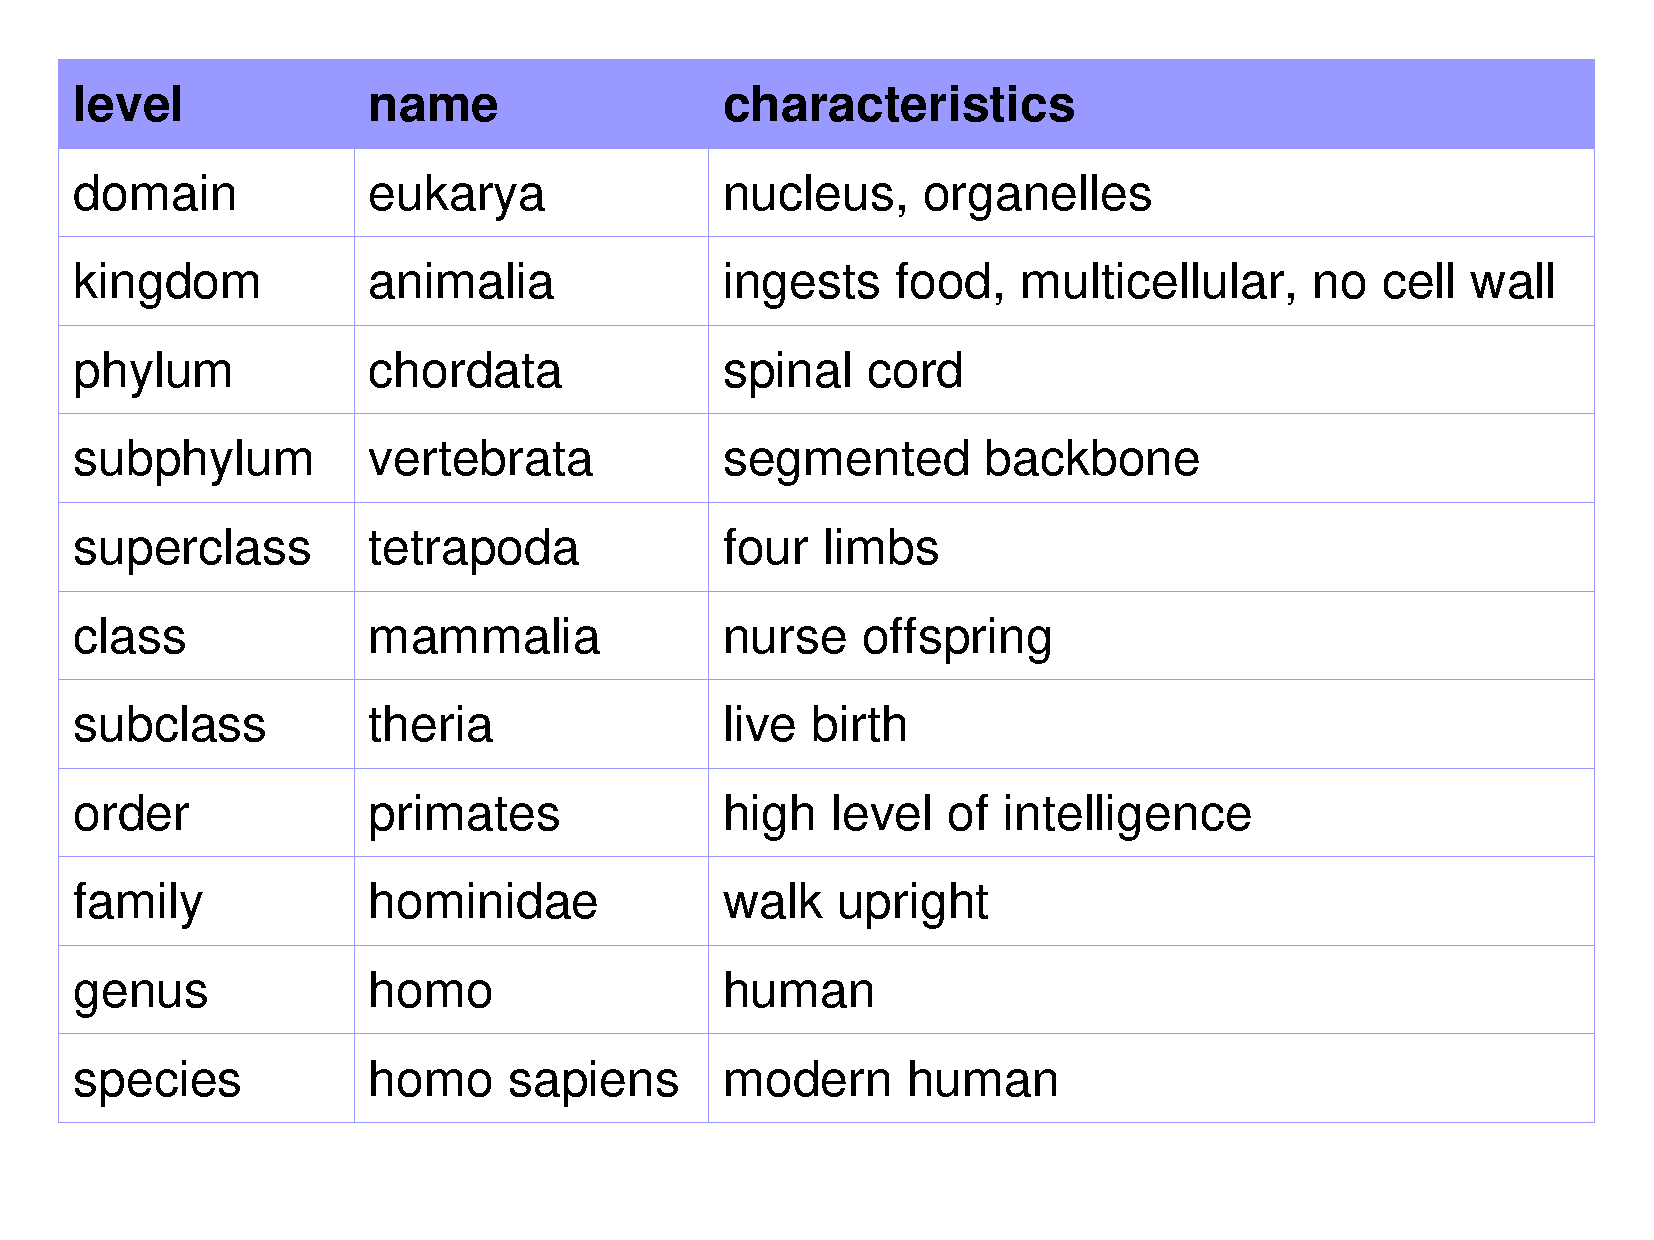
\includegraphics[scale=0.4,angle=-90]{graphic/taxonomy.pdf}
        \caption{Taxonomic Classification of the Animal Kingdom}
        \label{taxonomy_table}
    \end{center}
\end{table}

A very familiar example of an enumerated scheme is the traditional taxonomic
classification of the animal kingdom (figure \ref{taxonomy_table}). Most of the
existing medical terminologies, listing names of diseases, of surgical
operations and the like, are also enumerative. One example is the
\emph{International Classification of Diseases} (ICD) (chapter
\ref{res_medicinae_heading}).

After \cite{rogers}, attempting to enumerate in advance all useful phrases
inevitably encounters two serious problems concerning the \emph{Scale} and
\emph{Organisation}. Terminologies become:

\begin{enumerate}
    \item \emph{Scale:} too big to maintain, which results in inconsistent data
        that cannot be analysed anymore
    \item \emph{Organisation:} pre-categorised, which does not allow terms to
        be simultaneously placed under all different categories that are valid
\end{enumerate}

A further limitation is caused by unfavourable technical choices. The code often
serves two purposes. It is: the unique identifier of a concept and the means of
representing the relative organisation of a concept. So the common practice of
restricting the physical length of a code also restricts the levels of
organisation.

%
% $RCSfile: compositional_scheme.tex,v $
%
% Copyright (C) 2002-2008. Christian Heller.
%
% Permission is granted to copy, distribute and/or modify this document
% under the terms of the GNU Free Documentation License, Version 1.1 or
% any later version published by the Free Software Foundation; with no
% Invariant Sections, with no Front-Cover Texts and with no Back-Cover
% Texts. A copy of the license is included in the section entitled
% "GNU Free Documentation License".
%
% http://www.cybop.net
% - Cybernetics Oriented Programming -
%
% http://www.resmedicinae.org
% - Information in Medicine -
%
% Version: $Revision: 1.1 $ $Date: 2008-08-19 20:41:06 $ $Author: christian $
% Authors: Christian Heller <christian.heller@tuxtax.de>
%

\subsubsection{Compositional Scheme}
\label{compositional_scheme_heading}
\index{Compositional Scheme}
\index{Compositional Conceptual Scheme}
\index{Dictionary}
\index{Generalised Architecture for Languages, Encyclopedias and Nomenclatures in Med.}
\index{GALEN}
\index{Systematized Nomenclature of Medicine}
\index{SNOMED}
\index{Enumerative-compositional Scheme}
\index{Logical Observation Identifiers, Names and Codes}
\index{LOINC}
\index{International Classification of Nursing Procedures}
\index{ICNP}
\index{Combinatorial Explosion}

A \emph{Compositional Conceptual Scheme} typically contains a \emph{controlled}
and \emph{fixed} list (\emph{Dictionary}) of a relatively small number (a few
ten-thousand) of \emph{primitive} terms, each of which can have a unique code.
These primitives may be combined together by users to form more complex terms,
including those which might be found in an existing enumerative scheme but also
other, sometimes trivial, variations and expansions \cite{rogers}.

Examples of compositional schemes include the \emph{Generalised Architecture
for Languages, Encyclopaedias and Nomenclatures in Medicine} (GALEN) and the
\emph{Systematized Nomenclature of Medicine} (SNOMED). Hybrid
enumerative-compositional schemes are
\emph{Logical Observation Identifiers, Names and Codes} (LOINC) and the
\emph{International Classification of Nursing Procedures} (ICNP).

The sheer unlimited number of possible combinations, when seen as a problem, is
called \emph{Combinatorial Explosion}. Much worse problems, however, are the:

\begin{itemize}
    \item[-] \emph{Nonsense} combinations that may be constructed
        (avoidable with a set of semantic links, a grammar and constraints)
    \item[-] \emph{Redundancy} which occurs when more than one combination of
        terms express the same concept
        (avoidable with formal algorithms helping to identify redundant compositions)
    \item[-] \emph{Post-hoc Classification} (unforeseeable addition of new,
        unknown concepts) that may prevent a meaningful data analysis
        (avoidable with a type hierarchy of primitives and of semantics links)
    \item[-] \emph{Intractability} of data due to \emph{exploding} computer
        algorithms so that the computer will never find an answer
\end{itemize}

%
% $RCSfile: lexical_scheme.tex,v $
%
% Copyright (C) 2002-2008. Christian Heller.
%
% Permission is granted to copy, distribute and/or modify this document
% under the terms of the GNU Free Documentation License, Version 1.1 or
% any later version published by the Free Software Foundation; with no
% Invariant Sections, with no Front-Cover Texts and with no Back-Cover
% Texts. A copy of the license is included in the section entitled
% "GNU Free Documentation License".
%
% http://www.cybop.net
% - Cybernetics Oriented Programming -
%
% http://www.resmedicinae.org
% - Information in Medicine -
%
% Version: $Revision: 1.1 $ $Date: 2008-08-19 20:41:07 $ $Author: christian $
% Authors: Christian Heller <christian.heller@tuxtax.de>
%

\subsubsection{Lexical Scheme}
\label{lexical_scheme_heading}
\index{Lexical Scheme}
\index{Lexical Tech}
\index{Unified Medical Language System}
\index{UMLS}

A \emph{Lexical Technique} is one that helps compare phrases based on what they
appear to say -- on which words appear, in which order, and in what grammatical
constructs -- rather than on what they might or might not actually mean. Such
techniques can provide a powerful (but not 100\% accurate) method for mapping
between phrases in existing schemes, or between such phrases and the text found
in papers, the \emph{World Wide Web} (WWW) or other electronic resources.

One example of a lexical scheme is the \emph{Unified Medical Language System}
(UMLS).

Where lexical techniques break is when the language gets more \emph{slippery},
that is ambiguities may occur. Humans might interpret such results correctly,
but automated decision support systems would fail. Rogers \cite{rogers}
concludes that: \textit{As an input for autonomous machine processing
applications such as decision support, the outputs of natural language
processing tools remain unsuitable.}


%
% $RCSfile: ontology.tex,v $
%
% Copyright (c) 2001-2004. Christian Heller. All rights reserved.
%
% No copying, altering, distribution or any other actions concerning this
% document, except after explicit permission by the author!
% At some later point in time, this document is planned to be put under
% the GNU FDL license. For now, _everything_ is _restricted_ by the author.
%
% http://www.cybop.net
% - Cybernetics Oriented Programming -
%
% http://www.resmedicinae.org
% - Information in Medicine -
%
% @author Christian Heller <christian.heller@tuxtax.de>
%

\subsection{Ontology}
\label{ontology_heading}

Manifold definitions of the word \emph{Ontology} exist. They come from philosophy,
metaphysics, information technology and others -- too many to list here.
This document uses its own, adapted definition and considers an ontology to be
\emph{a strict hierarchy of abstract items, organized in levels of growing
granularity, that are solely unidirectionally related}. It such represents a
systematic description of complex domain contexts.

\begin{figure}[ht]
    \begin{center}
        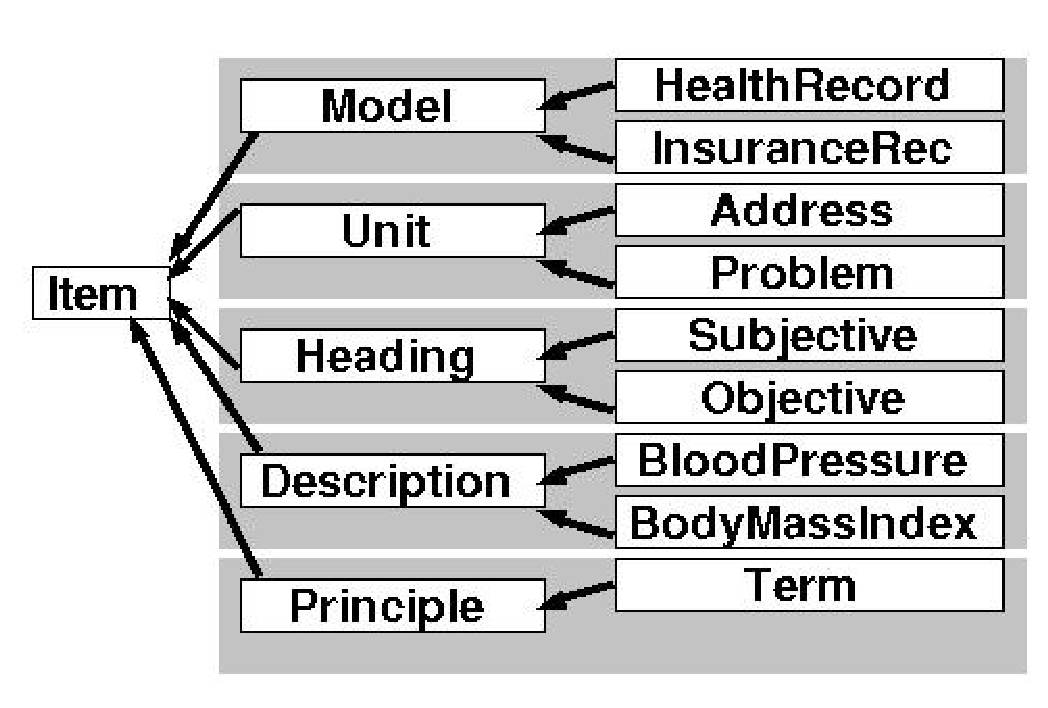
\includegraphics[scale=0.4]{vector/electronic_health_record_ontology.eps}
        \caption{Electronic Health Record Ontology}
        \label{electronic_health_record_ontology_figure}
    \end{center}
\end{figure}

Figure \ref{electronic_health_record_ontology_figure} shows one possible ontology
of an electronic health record, as described in the previous section.


%%
% $RCSfile: oio_form.tex,v $
%
% Copyright (C) 2002-2008. Christian Heller.
%
% Permission is granted to copy, distribute and/or modify this document
% under the terms of the GNU Free Documentation License, Version 1.1 or
% any later version published by the Free Software Foundation; with no
% Invariant Sections, with no Front-Cover Texts and with no Back-Cover
% Texts. A copy of the license is included in the section entitled
% "GNU Free Documentation License".
%
% http://www.cybop.net
% - Cybernetics Oriented Programming -
%
% http://www.resmedicinae.org
% - Information in Medicine -
%
% Version: $Revision: 1.1 $ $Date: 2008-08-19 20:41:07 $ $Author: christian $
% Authors: Christian Heller <christian.heller@tuxtax.de>
%

\subsection{OIO Form}
\label{oio_form_heading}

\emph{OIO Form}
Andrew Ho; OpenHealth Mailing List, December 2003 \cite{openhealth}

<form>
<item>
  <name>sBP</name>
  <description>systemic arterial blood pressure,supine</description>
  <prompt>sBP?</prompt>
  <itemtype>pressure</itemtype>
</item>
<itemtype>
  <name>pressure</name>
  <description>mmHg</description>
  <action>number</action>
  <choice></choice>
</itemtype>
</form>

OpenHealth Mailing List, December 2003 (relates to the OIO form above) \cite{openhealth}
Andrew Ho answers to Thomas Beale on the topic of OpenEHR Archetypes vs. OIO Forms

this form does not say anything about:
- systolic or diastolic (or other phases) of blood pressure
>
Just add it. Instead of "sBP" - call it "Systolic BP".
>
- what data type blood pressure is recorded as
>
The itemtype is "pressure". That is the "data type".
>
- what will you do if you want the patient standing - another form with
'standing' instead of 'supine'?
>
You can use another form or another item (a posture item).
>
- what if you want to record a time-series of BPs, say 3, with the patient
in a different position prior to each?
>
Just have 3 question items on the same form - or have 3 forms. Your choice.
>
- what if you want to record the protocol, i.e. instrument, cuff size
>
Add a question item called "protocol".
>
- how will you provide validation on data input, to e.g.
+ to ensure that
valid data types are used for each entered item (e.g. a Date is not entered
for diastolic BP)?
>
Use action=number
>
+ ensure that the systolic bp is in some sane range, e.g. 0-500mmHg?

Use action=number and choice='>20,<500', for example.
>
+ ensure that sensble positions of patient are offered to the user?

Communicate the "sensible positions" via the question prompt.
>
- how will you indicate that the data created by this form was in fact
created by this form (what is its id?), so that my software can process
the data according to the form's model of BP?
>
All data created via this OIO form are stored and labeled with the name of
this OIO form.

%
% $RCSfile: archetype.tex,v $
%
% Copyright (C) 2002-2008. Christian Heller.
%
% Permission is granted to copy, distribute and/or modify this document
% under the terms of the GNU Free Documentation License, Version 1.1 or
% any later version published by the Free Software Foundation; with no
% Invariant Sections, with no Front-Cover Texts and with no Back-Cover
% Texts. A copy of the license is included in the section entitled
% "GNU Free Documentation License".
%
% http://www.cybop.net
% - Cybernetics Oriented Programming -
%
% http://www.resmedicinae.org
% - Information in Medicine -
%
% Version: $Revision: 1.1 $ $Date: 2008-08-19 20:41:05 $ $Author: christian $
% Authors: Christian Heller <christian.heller@tuxtax.de>
%

\subsection{Archetype}
\label{archetype_heading}
\index{Archetype}
\index{Electronic Health Record}
\index{EHR}
\index{Good European/ EHR}
\index{GEHR}
\index{Open EHR}
\index{SNOMED CT}
\index{Archetype Definition Language}
\index{ADL}
\index{Constraint Form of ADL}
\index{cADL}
\index{Data Definition Form of ADL}
\index{dADL}
\index{Template Form of ADL}
\index{tADL}
\index{First Order Predicate Logic}
\index{FOPL}

With the aim of providing the means to build usable, maintainable, extensible
\emph{Electronic Health Records} (EHR), the \emph{Archetype} as design concept
was introduced in the \emph{Design Principles} document of the
\emph{Good European/ EHR} (GEHR) project, which was later renamed into
\emph{Open EHR} \cite{openehr}. Their website states: \textit{An archetype is a
re-usable, formal model of a domain concept.} Archetypes adhere to ontological
principles; they can be composed of other archetypes or atomic elements. Their
use is not limited to EHR building, despite OpenEHR's focus on the medical
domain.

Comparing archetypes with terminologies, Beale \cite{openehrtechnical} writes
that a terminology like for example SNOMED Clinical Terms (SNOMED CT) had the
form of a semantic network, i.e. \ldots\ with an ontological flavour. However,
because rigorous design principles were not always applied, they tended to be
internally inconsistent and had a lot of pre-coordination in them, while what
was really needed was a generative/ compositional terminology. Further, SNOMED
could tell what the meanings of the parts of e.g. a complete blood count test
are, but it were not going to provide a model of an actual blood test. This is
where archetypes \ldots\ would come in; they were about information
\emph{in use}, not definitions of reality (as terminologies). \ldots\ So --
even if SNOMED was perfect, it wouldn't do everything. It were a knowledge
support part of the environment, and it could be used to name things and
perform inferencing (\textit{draw a conclusion/ deduction} \cite{websters}).

An \emph{Archetype Definition Language} (ADL) \cite{adl} was created for the
specification of archetypes. A corresponding ADL document has the following
structure:

\begin{scriptsize}
    \begin{verbatim}
    archetype_id = <"some.archetype.id">
    adl_version = <"2.0">
    is_controlled = <True>
    parent_archetype_id = <"some.other.archetype.id">
    concept = <[concept_code]>
    original_language = <"lang">
    translations = <
    ...
    >
    description = <
    ...
    >
    definition = <
    cADL structural section
    >
    invariant = <
    assertions
    >
    ontology = <
    ...
    >
    revision_history = <
    ...
    >
    \end{verbatim}
\end{scriptsize}

Many separate sections can be identified in this archetype structure, and
various syntaxes are used for them. Table \ref{adl_table} gives an overview of
the structural elements of an ADL archetype. In addition to the single
sections, it mentions two further syntaxes, for templates and constraints on
data instances.

\begin{table}[ht]
    \begin{center}
        \begin{footnotesize}
        \begin{tabular}{| p{30mm} | p{30mm} | p{45mm} |}
            \hline
            \textbf{Element} & \textbf{Syntax} & \textbf{Purpose}\\
            \hline
            archetype structure & \emph{Archetype Definition Language} (ADL) & glue syntax\\
            \hline
            definition section & \emph{Constraint Form of ADL} (cADL) &
                constraints definition\\
            \hline
            description, ontology and other sections & \emph{Data Definition Form of ADL} (dADL) &
                data definition\\
            \hline
            template & \emph{Template Form of ADL} (tADL) &
                formalism to compose archetypes into larger constraint structures, used in particular contexts at runtime\\
            \hline
            data instances & \emph{First Order Predicate Logic} (FOPL) &
                constraints on data which are instances of some information model (e.g. expressed in UML)\\
            \hline
        \end{tabular}
        \end{footnotesize}
        \caption{Structural Elements of an ADL-defined Archetype \cite{adl}}
        \label{adl_table}
    \end{center}
\end{table}

Chapter \ref{cybernetics_oriented_language_heading} will define a new language
that is based on just one syntax: the \emph{Extensible Markup Language} (XML)
(section \ref{extensible_markup_language_heading}), an easy-to-grasp pure text
format. Despite its limited vocabulary of just four tags and four attributes,
that language may encode a rich set of knowledge constructs, including meta
information and constraints.

%
% $RCSfile: dual_model_approach.tex,v $
%
% Copyright (C) 2002-2008. Christian Heller.
%
% Permission is granted to copy, distribute and/or modify this document
% under the terms of the GNU Free Documentation License, Version 1.1 or
% any later version published by the Free Software Foundation; with no
% Invariant Sections, with no Front-Cover Texts and with no Back-Cover
% Texts. A copy of the license is included in the section entitled
% "GNU Free Documentation License".
%
% http://www.cybop.net
% - Cybernetics Oriented Programming -
%
% http://www.resmedicinae.org
% - Information in Medicine -
%
% Version: $Revision: 1.1 $ $Date: 2008-08-19 20:41:06 $ $Author: christian $
% Authors: Christian Heller <christian.heller@tuxtax.de>
%

\subsection{Dual Model Approach}
\label{dual_model_approach_heading}
\index{Dual Model Approach}
\index{Analysis Pattern}
\index{Two Level Modelling}
\index{Knowledge Level}
\index{Operational Level}
\index{Reflection Pattern}
\index{Meta Level}
\index{Base Level}
\index{Archetype Model}
\index{AM}
\index{Reference Model}
\index{RM}
\index{ADL}
\index{OpenEHR}

The idea of archetypes was inspired by Martin Fowler's \emph{Analysis Patterns}
\cite{fowler1997} describing a kind of ad hoc two-level modelling, using a
\emph{Knowledge Level} and \emph{Operational Level} -- as described by the
\emph{Reflection} pattern (section \ref{reflection_heading}), which calls the
two levels \emph{Meta Level} and \emph{Base Level}, respectively. Fowler tried
to put as much general domain knowledge as possible into the meta level, in
order to make application systems more flexible, and to remove unnecessary
dependencies. Archetypes represent what would traditionally have been put into
the knowledge (meta) level.

Because an \emph{Archetype Model} (AM) (defined in form of ADL documents) and
its runtime instances constrain a \emph{Reference Model} (RM) and its instances
(figure \ref{dual_figure}), development with archetypes is called the
\emph{Dual Model Approach} \cite{openehr}. Archetypes represent the knowledge
belonging to the meta level; the reference model contains information belonging
to the base level. \textit{RMs are domain-invariant, i.e. the concepts
expressed in the base models mean the same thing right across the domain.}
\cite[Beale]{openehrtechnical}

\begin{figure}[ht]
    \begin{center}
        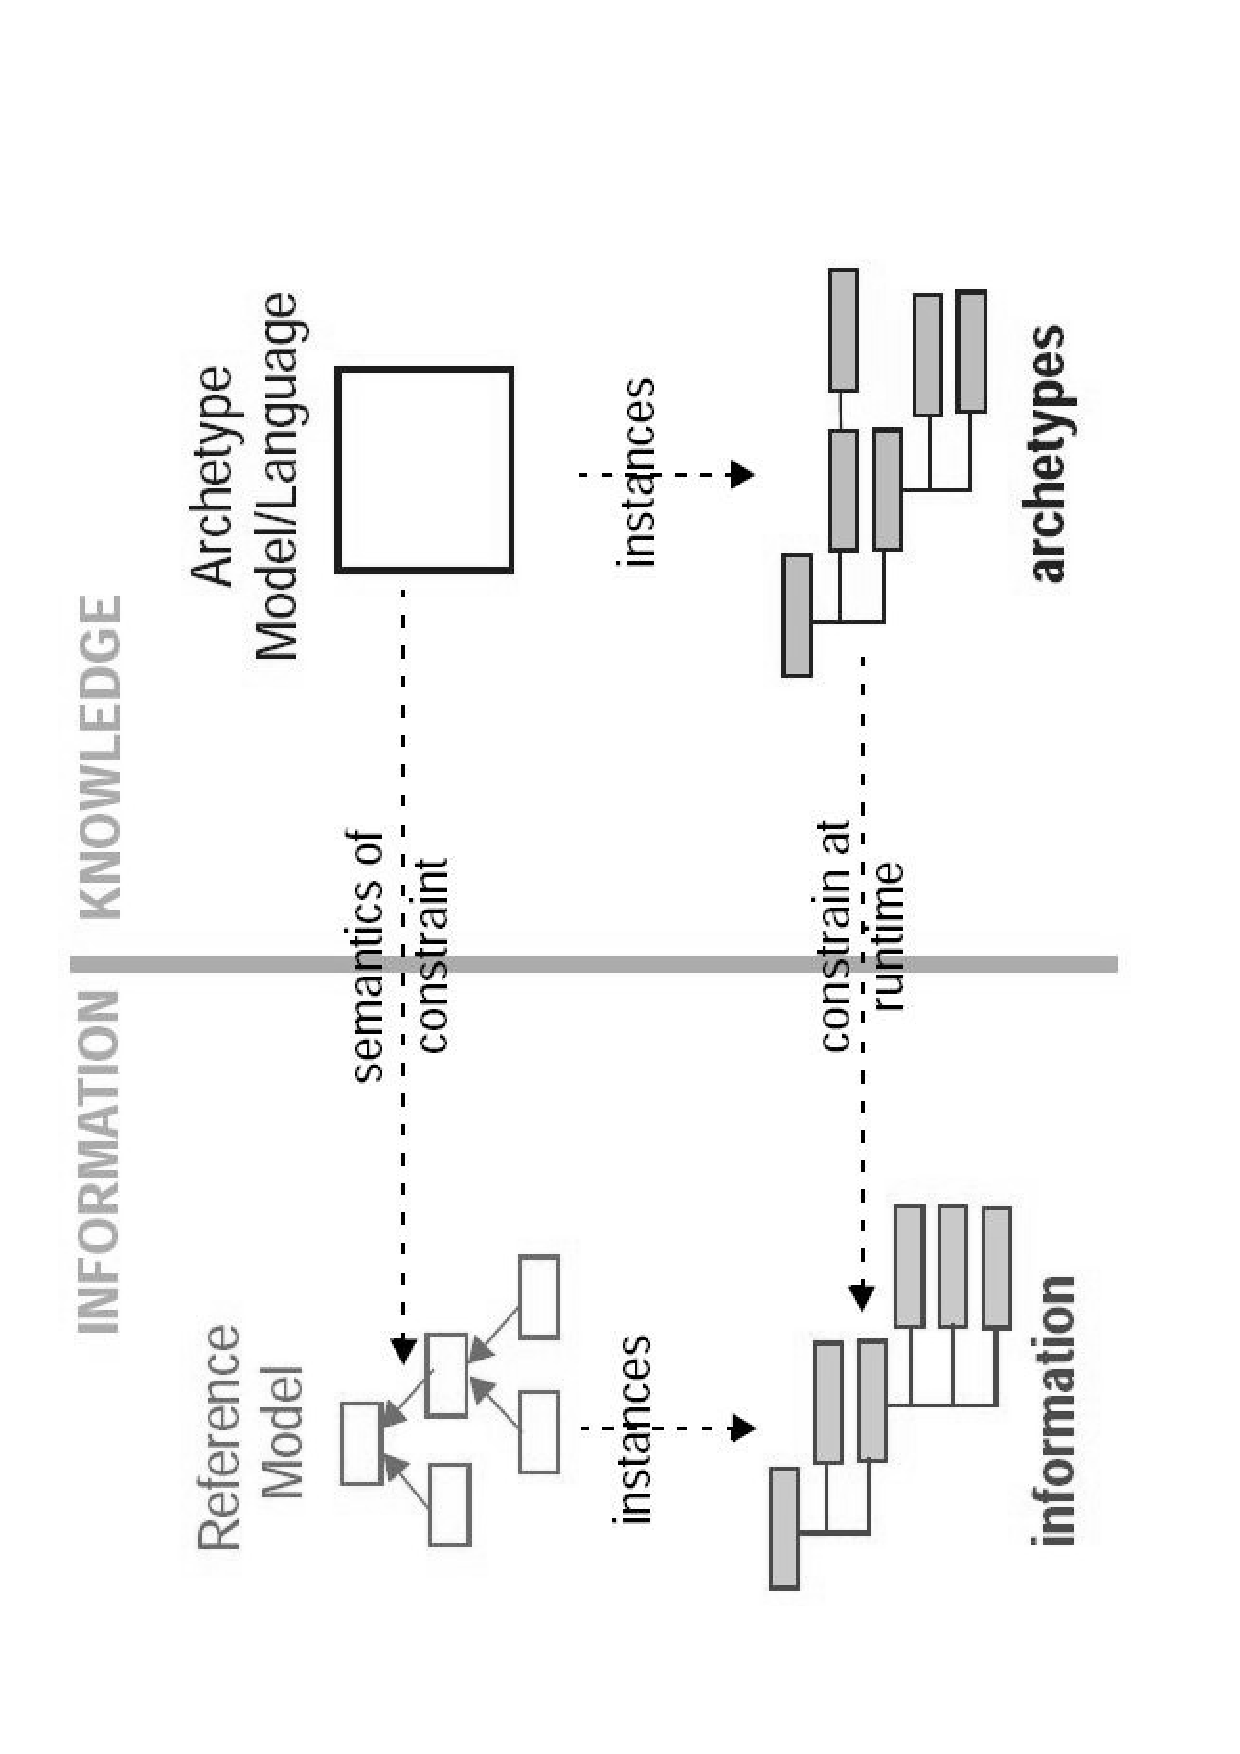
\includegraphics[scale=0.3,angle=-90]{graphic/dual.pdf}
        \caption{Dual Model Approach \cite{archetypes}}
        \label{dual_figure}
    \end{center}
\end{figure}

The difference between the dual model approach and classical meta architectures
is that the latter implement both, meta- and base level using the same
technology (language). Archetypes, on the other hand, use the ADL for
specifying knowledge. Further, the AM does not depend on the RM, as opposed to
meta architectures, where both models depend on each other bidirectionally.
Ergo, the dual model approach is rather comparable to \emph{Agents} (section
\ref{agent_oriented_programming_heading}) owning a mental state (knowledge base).

There are unclear views on what exactly should be constrained when. Sam Heard
\cite{openehrtechnical} writes about an \emph{Archetype Kernel} -- a tool that
could help build (knowledge instances) and ensure that (they) comply to
archetypes \ldots\ It could operate at a range of points, at:

\begin{itemize}
    \item[a] write and edit time: allowing constraint of the data to be based
        on archetypes (metadata) rather than application specific processes;
    \item[b] creation time of the application or schema: so that the
        application has read all information constraining the data as indicated
        -- but not through interaction with the archetype at runtime;
    \item[c] persistence time: into a database or some other persistence means;
    \item[d] communication time: such as when creating a model extract.
\end{itemize}

Besides obvious benefits of these approaches in constraining domain knowledge,
there are a number of potential problems, as Heard mentions:

\begin{quote}
    \emph{a} makes \emph{b} and \emph{c} redundant and allows the application
    to stay up to date with the archetype development process; \emph{b} makes
    \emph{c} redundant (potentially) but means code has to be cut to
    encorporate new archetypes; \emph{c} and \emph{d} mean that data may be
    proved incompatible at a time later than data entry and this may lead to
    other problems; \emph{d} means you can carry on regardless but there is a
    risk that data collected will not be compatible with models that are
    proposed for interoperability.
\end{quote}

Further weaknesses of archetypes, the ADL and dual model approach are:

\begin{itemize}
    \item[-] mix of meta information (properties, constraints) and hierarchical whole-part structure in ADL
    \item[-] incomplete domain knowledge in ADL lacking logic (algorithms/ workflows) and user interfaces
    \item[-] inflexible structures due to runtime-dependency of RM instances from archetypes
    \item[-] use of object-oriented concepts with all their limits, for RM as well as for AM instances
\end{itemize}

Although the \emph{OpenEHR} project \cite{openehr} claims archetypes to be both:

\begin{enumerate}
    \item[-] \emph{domain-empowered:} domain experts, rather than information
        technology people, become able to directly define and manage the
        knowledge definitions of their systems;
    \item[-] \emph{future-proof:} systems can be deployed prior to having
        created formal knowledge models of the (entire) domain
\end{enumerate}

\ldots\ the above-mentioned issues prevent them from being so. The dual model
approach in conjunction with archetypes only partly fulfills the expectations
of independent and complete knowledge structures. CYBOP sets out to solve these
issues and to find a truely future-proof, long-life system architecture.
Knowledge templates written in the language described later in this work
(chapter \ref{cybernetics_oriented_language_heading}) may not only contain meta
information constraining application models (as archetypes do), they represent
the application itself. The templates themselves are constrained at design time
through one universal knowledge schema (chapter \ref{knowledge_schema_heading})
dictating their structure. Runtime knowledge models do not reference the
template they were instantiated with (contrary to RM instances referencing
their corresponding AM instance); a CYBOP application holds all constraints
directly in its knowledge models (runtime instances). Since these models follow
the structure of the singular knowledge schema as well, they can be serialised
easily what makes further constrain activities for persistence or communication
unnecessary.

